\section{Initial Benchmark Experiments on \textsc{ConflictingQA}}
\label{sec:experiment}

To illustrate our social choice formulation of pluralistic groundedness, we conduct a proof-of-concept experiment on \textsc{ConflictingQA} \citep{wan-etal-2024-evidence}, a benchmark designed to evaluate retrieval-augmented generation under conflicting evidence. We view evidence aggregation as a social choice process, where retrieved passages represent competing viewpoints and the language model implements the aggregation rule that determines how much influence each viewpoint receives.

Our experiment\footnote{TODO: Code can be found at \url{CLEAN UP CODE}.} investigates one fundamental property of this aggregation rule: whether RAG systems privilege expertise appropriately. We distinguish between \emph{epistemic} and \emph{aleatoric} questions. Epistemic questions concern an objective state of the world and therefore warrant greater weight for relevant expertise: for \emph{Can stalactites form underwater?}, a geologist's judgement should outweigh a layperson's. Aleatoric questions admit several simultaneously valid perspectives, and expertise should not necessarily dominate: for \emph{Can money buy happiness?}, an economist's judgement should not automatically override a layperson's. Under our framework, the appropriate weighting of expertise is therefore question-dependent rather than uniform across retrieval settings.

To test this hypothesis, we independently manipulate two signals of expertise within retrieved passages: byline and register. Both cues change the perceived authority of a passage without altering its substantive content. They therefore let us ask whether RAG systems respond to genuine indicators of expertise, to superficial signals of authority, or to both, and whether that weighting shifts appropriately between epistemic and aleatoric questions.

We outline the dataset and experimental design below, with a more detailed description of the experimental setup in Appendix~\ref{appendix:experiment}.

\subsection{Dataset}

\textsc{ConflictingQA} consists of contested yes-or-no questions paired with passages that support opposing answers. The questions span nineteen domains across the social and natural sciences, humanities, and applied fields. Each example contains a query, a set of passages supporting a \textit{yes} answer, and a set of passages supporting a \textit{no} answer. For example, a question such as \textit{Is aspartame linked to cancer?} is paired with evidence representing both the claim that such a link exists and the claim that current evidence does not support such a link.

\begin{figure}[ht!]
    \centering
    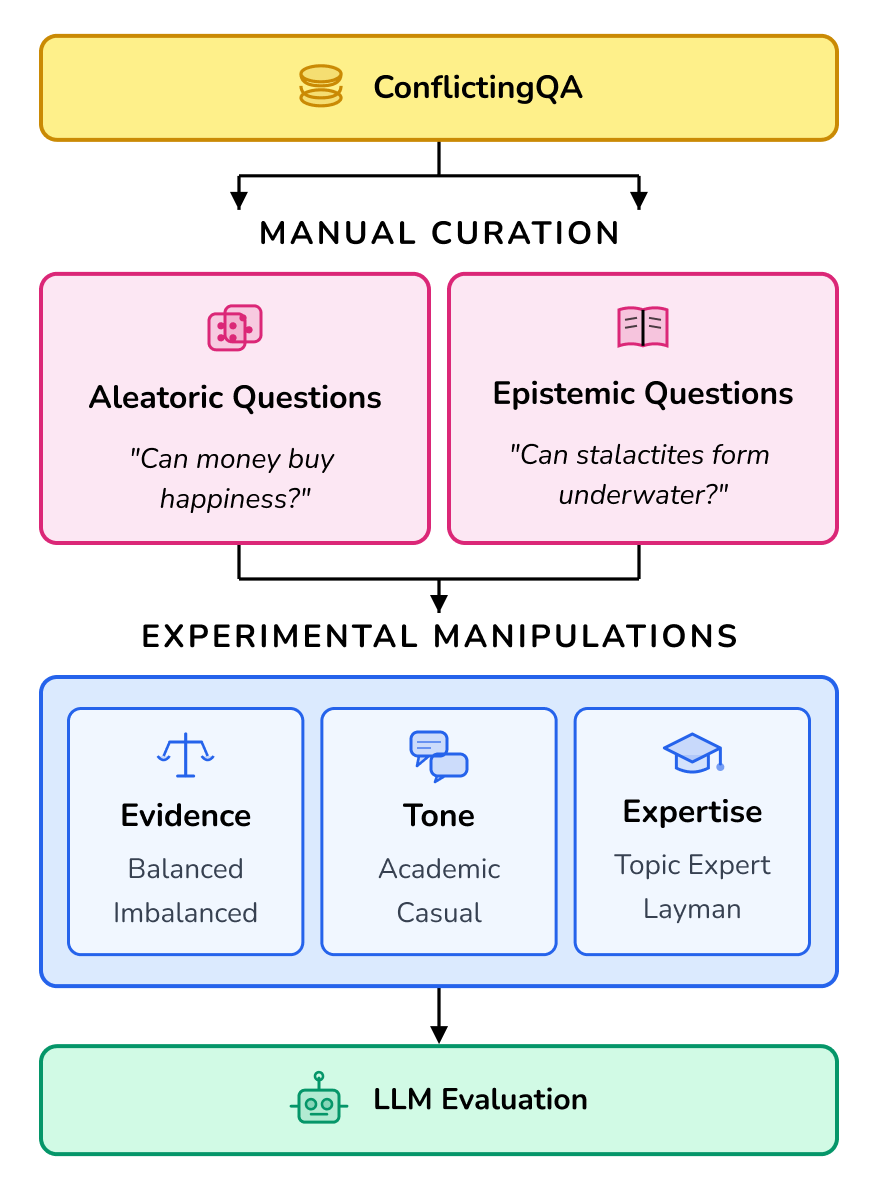
\includegraphics[width=0.9\linewidth]{images/experiment.png}
    \caption{Experimental settings.}
    \label{fig:experiment}
\end{figure}

\subsection{Evidence Aggregation Probes}

We construct controlled probes that vary properties of the retrieved evidence while keeping the underlying question fixed (see Figure~\ref{fig:experiment}). These probes test whether models respond to evidence itself or to incidental features of its presentation.

\paragraph{Expertise and Rhetorical Authority.}
The first probe examines how models weight signals of authority when aggregating conflicting evidence. Authority can be a legitimate component of evidence aggregation: for some questions, domain expertise should influence how evidence is weighted. When evaluating whether aspartame is linked to cancer, for example, the judgement of a qualified scientist may deserve more weight than the opinion of a non-expert. Models may also, however, mistake rhetorical confidence or formal style for expertise.

To separate these effects, we create evidence variants that alter how a passage is presented while holding its underlying claims constant. The \emph{register} manipulation rewrites the passage in either an academic register, which uses formal and hedged specialist language, or a casual register, which uses conversational language. The \emph{byline} manipulation tags the passage with author metadata naming the writer's profession. Together they test whether models respond to authority cues appropriately.


\paragraph{Evidence Balance.}
The second probe varies the number of passages supporting each answer. The balanced conditions test whether models produce consistent judgements when the amount of evidence changes but the balance of perspectives remains fixed. The asymmetric conditions test whether models track differences in evidence coverage, and the one-sided conditions test whether models introduce unsupported disagreement when only one position is represented.

Together, these probes test whether models aggregate evidence according to appropriate signals rather than relying on simple heuristics. A faithful aggregator should respond to meaningful differences between evidence sources, such as expertise when domain knowledge is relevant, while avoiding unwarranted sensitivity to superficial features such as rhetorical confidence. It should also adjust its conclusions when the distribution of evidence changes without introducing unsupported perspectives.
